% !TeX root = ../main.tex
% Add the above to each chapter to make compiling the PDF easier in some editors.

\chapter{Software Application}\label{Software Application}

\section{Methodolgy}
The main focus is to develop a low-cost mobile system to locate and examine veins. As one can infer from the design of the hardware extension from the previous chapter, the cost of the hardware components is mainly the cost of a normal webcam, NIR-pass filter, a PCB breadboard and a set of NIR LEDs. Obviously, the cost of these elements is very low (under 30 Euros). The second component is the software application. In order to maintain the low-cost constraint, the software application must be run on normal android mobiles or tablets. Not on special hardware or expensive embedded systems.

\subsection{Control of Hardware Extension}

The hardware extension is connected as a peripheral to an android device. In that sense, the android device takes over control of the hardware peripheral in somehow. This control can be described as power control and camera control.

\subsubsection{Power Control}
Only a single connection via OTG cable is needed. Data and power are then transferred using the data and power pins of the OTG connection respectively. Power is supplied whenever the OTG cable is plugged in. No programmable way for cutting off power was implemented. Because turning off the host port’s power needs write permission on the \texttt{/sys} directory and this cannot be acquired without root. The application is developed to be fully runnable on not rooted devices, so it requires no root access. For these reasons, controlling the OTG connection programmatically was out of the scope of this project. Of course, a physical switch can be also added on the whole circuit to turn the system on or off. 

\subsubsection{Camera Control}

A third-party library, UVC Camera library, was used in this project to enable the android device to communicate with the webcam. UVC Camera supports variety of camera properties control like brightness, contrast, focus control and more, given that the camera itself supports those. Support is indicated by flags that the camera provides. Control of such properties can be done in the C++ side. Signals are sent from the module to the camera to change sensor values. For example, brightness and contrast control were added in the project. In this case, brightness and contrast are controlled by changing some sensor values, without the need of using image processing at all.


As per the UVC specification, if the auto setting is supported and set to the on state, the device will provide automatic focus adjustment, and read requests will reflect the automatically set value \parencite{uvcCamera}. Attempts to programmatically set the Focus control are ignored when auto mode is set. When the UVC Camera library detects an autofocus support in a connected webcam, it uses it and sets the autofocus mode.



\subsection{Vein Visualization Enhancement}

In our setting, raw videos that come directly from the NIR camera provide good visualization of the vein’s structure and their pattern. However, they contain some fuzzy and noisy areas caused by shades or hairs.

Veins visualization can be enhanced more using image processing or machine learning.
Videos received by a camera are made up from a succession of still frames and are then played one after the other several times a second. Image enhancement algorithms can be applied on each frame separately each time a new frame arrives from the camera. The result is then displayed in the real time on the screen.


\subsubsection{Image Processing}



\subsubsection{Machine Learning}



\subsubsection{Conclusion}

\subsection{Application Work Modes}






\section{Application Structure}
The software application is basically an android application composed of two layers: the native layer, written in C++ and the Java layer. 
The Java layer includes user interface (UI) components of the application and all application business logic. 
The C++ layer is responsible for communicating with the camera as well as for image processing of raw images coming from the camera using open computer vision library (OpenCV).

Because compiled Java code runs on the Java virtual machine (JVM) which is a part of the Java runtime environment (JRE). Whereas compiled C++ runs directly on the operating system (OS), a bridging component Between the two layers is needed.
The Java native interface (JNI) allows the two layers to interact with each other. It is a Java feature that allows Java code to call native applications and libraries written in languages such as C, C++ and Objective-C.

The \autoref{fig:applicationArchitecture} below shows the application high-level architecture.


\begin{figure}[H]
\centering
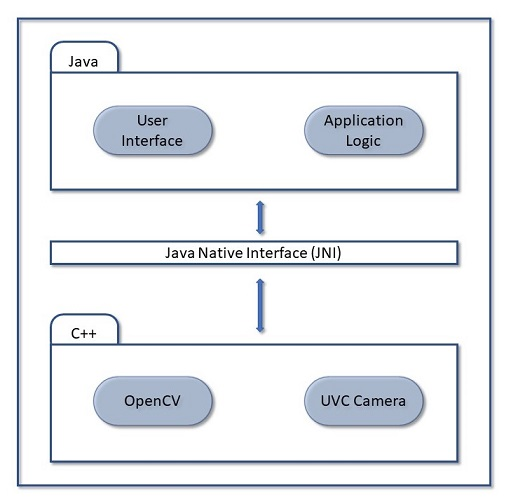
\includegraphics{figures/applicationArchitecture.JPG}
\caption[Application architecture]{Application architecture}\label{fig:applicationArchitecture}
\end{figure}


\section{C++ Layer}


C++ is a highly flexible and adaptable language. Since its creation, it has been used for a wide variety of programs including firmware for micro-controllers, operating systems, applications, and graphics programming \parencite{cpp}.

Written in C++, this application layer encompasses the UVC driver library which allows the application to communicate with the camera as well as the native image processing module, the OpenCV module.

\subsection{USB Video Class}

USB Video Class (UVC) describes the capabilities and characteristics of video streaming devices. It is widely used, such as desktop video cameras or webcams, digital camcorders, still-image cameras, and so forth. USB Video Class (UVC) is a standard class specification that standardizes video streaming functionality on the USB. It enables devices like webcams, digital camcorders, analog video converters, analog and digital television tuners etc to connect seamlessly with host machines. UVC supports streaming multiple video formats and provides structures for describing the functionalities of the video device to the host and defines USB requests to control different parameters of the device and characteristics of the video stream. It also provides flexibility for a video device to support multiple video resolutions, formats and frame rates, which highly influences the bandwidth negotiation between the device and the host \parencite{uvc}.

\subsection{UVC Camera Library for Android}
Many OS platforms have native support for UVC drivers which greatly reduces the time required for developers to connect UVC devices. Unfortunately, android doesn’t offer such a support, therefore, to connect a UVC device such as a webcam, the device driver must be written by the developer. 
Nevertheless, third-party and open source libraries offer good alternative solution for the UVC device drivers. An open source library to access to UVC webcams on non-rooted Android device called UVCCamera was used in this project \parencite{uvcCamera}. The library works on minimum android version 3.1 or later (API >= 12), but Android 4.0(API >= 14) or later is recommended.


\subsubsection{Open Computer Vision Library}
OpenCV is written in C and C++ and runs under Linux, Windows and Mac OS X. OpenCV was designed for computational efficiency and with a strong focus on realtime applications. OpenCV is written in optimized C and can take advantage of multicore processors. One of OpenCV’s goals is to provide a simple-to-use computer vision infrastructure that helps people build fairly sophisticated vision applications quickly \parencite{openCv}.



\section{Java Layer}


The compiled Java code along with any data and resource files required by the application is bundled by the android asset packaging tool (AAPT) tool into an android package, an archive file marked by an .apk suffix.
The Java layer includes the user interface (UI) components and all application buisness logic.

\subsection{Permissions}
\subsubsection{USB Host}
By default, Android does not allow an application to access the devices connected to the USB  port. To enable an application to interact with a the UVC camera directly connected by OTG cable, this functionality must be declared by adding the \texttt{<uses-feature android:name="android.hardware.usb.host"/>} tag in the manifest section in\texttt{AndroidManifest.xml}. 

\subsubsection{Open GL}

OpenGL ES (Open Graphics Library for Embedded Systems) is an API to graphics hardware. The API consists of a set of several hundred procedures and functions that allow a programmer to specify the shader programs, objects and operations involved in producing high-quality graphical images, specifically color images of three-dimensional objects\parencite{openGl}.


Android includes support for high performance 2D and 3D graphics with the OpenGL ES. Similar to USB host permission, adding  \texttt{<uses-feature android:glEsVersion="0x0\\0030000"/>} tag to include OpenGL ES support is needed. This tells android to expect the version 3 of OpenGL ES.








 
